\documentclass{standalone}

\usepackage{tikz}

\begin{document}
	
	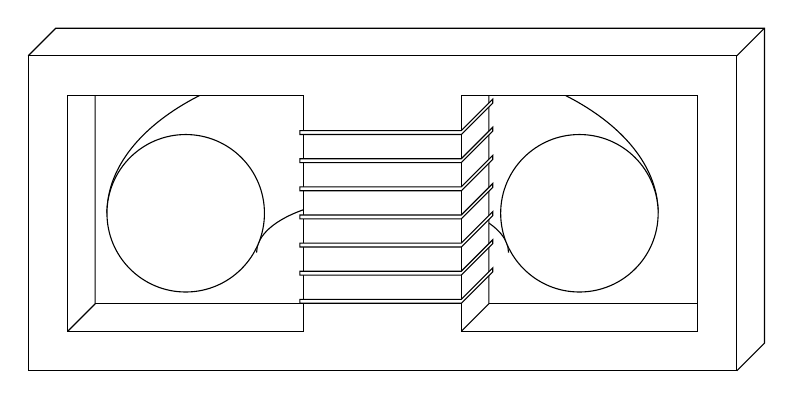
\begin{tikzpicture}
	
		\def\Rx{3.5}
		\def\Ry{2}
		\def\rx{1.6}
		\def\ry{0.7}
		
		\def\cx{2.5}
		\def\cy{0}
		    
		    % Dessin du tokamak
		    \draw (\Rx,\cy) [x radius=\Rx cm, y radius=\Ry .cm] 
    arc[start angle=0, end angle=180];
    
    		 \draw (\rx,\cy-0.5) [x radius=\rx cm, y radius=\ry cm] 
    arc[start angle=0, end angle=180];
    
    \def\R{1}
    
		    \draw[fill=white] (-\cx,\cy) ellipse [x radius=\R cm, y radius=\R cm];
		
		    \draw[fill=white] (\cx,\cy) ellipse [x radius=\R cm, y radius=\R cm];
		    
		    % On efface ce qui va être recouvert
		    
		    \def\Shift{0.5}
		    \def\shift{0.35}
		    
		    \fill[white] (-\R, -\R-\Shift) -- (-\R, \R+\Shift) -- (-\cx-\R-\Shift, \cy+\R+\Shift) -- (-\cx-\R-\Shift, \cy+\R+2*\Shift) -- (\cx+\R+\Shift, \cy+\R+2*\Shift) -- (\cx+\R+\Shift, \cy+\R+\Shift) -- (\R, \cy+\R+\Shift) -- (\R, -\cy-\R-\Shift) -- cycle;
		    
		    		    \fill[white] (\R, -\R-\Shift) -- (\R+\shift, -\R-\shift) -- (\R+\shift, \R+\Shift) -- (\R, \R+\Shift) -- cycle;
		    		    
		    % Dessine les bord de l'ion core
		    
		    \draw (-\cx-\R-\Shift, \R+\Shift) -- (-\R, \R+\Shift) -- (-\R, -\R-\Shift) -- (-\cx-\R-\Shift, -\R-\Shift) -- cycle;
		    
		    \draw (-\cx-\R-\Shift, -\R-\Shift) -- (-\cx-\R-\Shift+\shift, -\R-\Shift+\shift) -- (-\cx-\R-\Shift+\shift, \R+\Shift);
		    \draw (-\cx-\R-\Shift+\shift, -\R-\Shift+\shift) -- (-\R, -\R-\Shift+\shift);
		    
		    \draw (\cx+\R+\Shift, \R+\Shift) -- (\R, \R+\Shift) -- (\R, -\R-\Shift) -- (\cx+\R+\Shift, -\R-\Shift) -- cycle;
		    

		    \draw (\R, -\R-\Shift) -- (\R+\shift, -\R-\Shift+\shift) -- (\R+\shift, \R+\Shift);
		    \draw (\R+\shift, -\R-\Shift+\shift) -- (\cx+\R+\Shift, -\R-\Shift+\shift);
		    
		    \draw (-\cx-\R-2*\Shift, \R+2*\Shift) -- (\cx+\R+2*\Shift, \R+2*\Shift) -- (\cx+\R+2*\Shift, -\R-2*\Shift) -- (-\cx-\R-2*\Shift, -\R-2*\Shift) -- cycle;
		    \draw (-\cx-\R-2*\Shift, \R+2*\Shift) -- (-\cx-\R-2*\Shift+\shift, \R+2*\Shift+\shift) -- (\cx+\R+2*\Shift+\shift, \R+2*\Shift+\shift) -- (\cx+\R+2*\Shift+\shift, -\R-2*\Shift+\shift) -- (\cx+\R+2*\Shift, -\R-2*\Shift);
		    \draw (\cx+\R+2*\Shift+\shift, \R+2*\Shift+\shift) -- (\cx+\R+2*\Shift, \R+2*\Shift);
		    
		    % Primary winding

			\def\elong{0.05};
			\def\n{7};
		    
		    \foreach \i in {1,...,\n}{

    \fill[white]
        (-\R-\elong, -\R-\Shift+\i*\Shift/\n+\i*2*\R/\n)
        -- (\R, -\R-\Shift+\i*\Shift/\n+\i*2*\R/\n)
        -- (\R+\shift+\elong, -\R-\Shift+\i*\Shift/\n+\i*2*\R/\n+\shift+\elong)
        -- (\R+\shift+\elong, -\R-\Shift+\i*\Shift/\n+\i*2*\R/\n+\shift+2*\elong)
        -- (\R, -\R-\Shift+\i*\Shift/\n+\i*2*\R/\n+\elong)
        -- (-\R-\elong, -\R-\Shift+\i*\Shift/\n+\i*2*\R/\n+\elong)
        -- cycle;

    \draw
        (-\R-\elong, -\R-\Shift+\i*\Shift/\n+\i*2*\R/\n)
        -- (\R, -\R-\Shift+\i*\Shift/\n+\i*2*\R/\n)
        -- (\R+\shift+\elong, -\R-\Shift+\i*\Shift/\n+\i*2*\R/\n+\shift+\elong)
        -- (\R+\shift+\elong, -\R-\Shift+\i*\Shift/\n+\i*2*\R/\n+\shift+2*\elong)
        -- (\R, -\R-\Shift+\i*\Shift/\n+\i*2*\R/\n+\elong)
        -- (-\R-\elong, -\R-\Shift+\i*\Shift/\n+\i*2*\R/\n+\elong)
        -- cycle;
}
	
	\end{tikzpicture}	
	
\end{document}